\begin{frame}{Random Variables}
    \begin{itemize}
        \item We often model processes using what's called random variables.
        \item Random variables give us a mathematical framework for working with real-world variables.
        \item This allows us to make predictions and statistical inference.
    \end{itemize}
\end{frame}

\begin{frame}{Example: Textbooks}
    Two books are assigned for a statistics class: a textbook and its corresponding study guide. The university bookstore determined that
    \begin{itemize}
        \item 20\% of enrolled students do not buy either book
        \item 55\% buy the textbook only
        \item 25\% buy both books
    \end{itemize}
    If there are 100 students enrolled, how many books should the bookstore expect to sell to this class?
\end{frame}

\begin{frame}{Example: Textbooks}
    If there are 100 students enrolled, how many books should the bookstore expect to sell to this class?
    \begin{itemize}
        \item Around $100\times0.20=20$ students will buy neither book (0 books sold).
        \item Around $100\times0.55=55$ students will buy the textbook only (55 books sold).
        \item Around $100\times0.25$ students will buy both books (50 books sold).
    \end{itemize}
    The bookstore should expect to sell about $55+50=105$ books for this class.
\end{frame}

\begin{frame}{Example: Textbook}
    Now suppose the textbook costs \$137 and the study guide \$33. How much revenue should the bookstore expect from this class of 100 students?
    
    \begin{itemize}
        \item A student who buys only the textbook spends \$137.
        \begin{itemize}
            \item We expected about 55 students to buy the textbook only, for a total of $\$137\times 55 = \$7535$
        \end{itemize}
        \item A student who buys both books spends $\$137 + \$33 = \$170$
        \begin{itemize}
            \item We expected about 25 students to buy both books, for a total of $\$170\times 25=\$4250$
        \end{itemize}
    \end{itemize}
\end{frame}

\begin{frame}{Example: Textbook}
    Now suppose the textbook costs \$137 and the study guide \$33. How much revenue should the bookstore expect from this class of 100 students?
    
    \begin{itemize}
        \item In total, the bookstore can expect $\$7535+\$4250=\$11785$ from this class each term. 
        \item However, some \textit{sampling variability} will cause this number to differ slightly each term.
    \end{itemize}
\end{frame}

\begin{frame}{Expectation}
    \begin{itemize}
        \item We call a variable or process with a numerical outcome a \textbf{random variable}.
        \item We usually represent random variables with capital letters such as $X$, $Y$, or $Z$. 
        \item The amount of money a single student will spend on her statistics books is a random variable. We might represent it by $X$.
    \end{itemize}
\end{frame}

\begin{frame}{Expectation}
    \begin{itemize}
        \item The possible outcomes of $X$ are labeled with a corresponding lower case letter $x$ and subscripts.
        \item For our textbook example, we would write
        \begin{itemize}
            \item $x_1=\$0$
            \item $x_2=\$137$
            \item $x_3=\$170$
        \end{itemize}
    \end{itemize}
\end{frame}

\begin{frame}{Expectation}
    \begin{itemize}
        \item The corresponding probabilities may be written as
        \begin{itemize}
            \item $P(X=x_1)=P(X=\$0)=0.20$
            \item $P(X=x_2)=P(X=\$137)=0.55$
            \item $P(X=x_3)=P(X=\$170)=0.25$
        \end{itemize}
    \end{itemize}
\end{frame}

\begin{frame}{Expectation}
    The probability distribution for $X$ looks like
    \begin{center}
        \begin{tabular}{l ccc r}
            \hline
            $i$ & 1 & 2 & 3 & Total \\ \hline
            $x_i$ & \$0 & \$137 & \$170 & - \\
            $P(X=x_i)$ & 0.20 & 0.55 & 0.25 & 1.00 \\ \hline
        \end{tabular}
    \end{center}
\end{frame}

\begin{frame}{Expectation}
    Previously, we computed the average outcome of $X$ as \$117.85.
    \begin{itemize}
        \item We call this average outcome the \textbf{expected value} of $X$, denoted $E(X)$.
        \item The expected value of a random variable is computed by adding each outcome weighted by its probability.
    \end{itemize}
    \begin{align*}
        E(X) &= 0\times P(X =0)+137\times P(X =137)+170\times P(X =170) \\
        &= 0 \times 0.20 + 137 \times 0.55 + 170 \times 0.25 \\
        &= 117.85
    \end{align*}
\end{frame}

\begin{frame}{Expected Value of a Discrete Random Variable}
    If $X$ takes outcomes $x_1, \dots, x_k$ with probabilities $P(X = x_1), \dots, P(X = x_k)$, the expected value of $X$ is the sum of each outcome multiplied by its corresponding probability:
    \begin{align*}
        E(X)&=x_1 \times P(X =x_1)+\dots +x_k ×P(X =x_k) \\
        &= \sum_{i=1}^k x_i P(X=x_i)
    \end{align*}
\end{frame}

\begin{frame}{Expected Values}
    \begin{itemize}
        \item The expected value for a random variable represents the average outcome. 
        \item For example, E(X) = 117.85 represents the average amount the bookstore expects to make from a single student.
        \item You will occasionally see the expected value denoted as $\mu$. We will explore how this relates to the true/population mean as we go.
    \end{itemize}
\end{frame}

\begin{frame}{Expected Value of a Continuous Random Variable}
    \begin{center}
        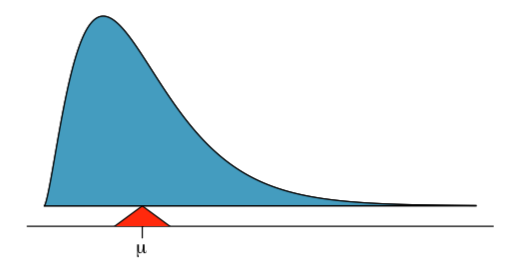
\includegraphics[scale=0.4]{images/contdist.png}
    \end{center}
    
    \vspace{-20pt}\begin{itemize}
        \item We can also calculate the expected value for a continuous random variable. 
        \item This requires a little bit of calculus, so we won't require it for this course.
        \item If you are familiar with Riemann sums and integrals, this is a similar transition from discrete to continuous.
    \end{itemize}
\end{frame}

\begin{frame}{Variability in Random Variables}
    For the bookstore looking at textbook revenues, it might also be of interest to know about the variability in revenue.
    \begin{itemize}
        \item The variance and standard deviation can be used to describe the variability of a random variable.
        \item We talked about calculating variance as the sum of the squared deviances from the mean. 
    \end{itemize}
\end{frame}

\begin{frame}{Variability in Random Variables}
    For the bookstore looking at textbook revenues, it might also be of interest to know about the variability in revenue.
    \begin{itemize}
        \item Calculating a variance for a random variable is similar, but now we weight each squared deviance by its corresponding probability.
        \item This is somewhere in between the variance formula we talked about in Chapter 2 and the weighting we used for the expected value.
        \item We again calculate the standard deviation as the square root of the variance. 
    \end{itemize}
\end{frame}

\begin{frame}{Variance Formula}
    If $X$ takes outcomes $x_1, \dots, x_k$ with probabilities $P(X = x_1), \dots, P(X = x_k)$ and expected value $\mu=E(X)$, then the variance of $X$, denoted by $Var(X)$ or $\sigma^2$, is
    \begin{align*}
        Var(X) &= (x_1−\mu)^2\times P(X=x_1)+\dots + (x_k − \mu)^2 \times P (X = x_k ) \\
        &= \sum_{j=1}^k (x_j - \mu)^2 P(X=x_j)
    \end{align*}
    The standard deviation of $X$, labeled $sd(X)$ or $\sigma$, is the square root of the variance.
\end{frame}

\begin{frame}{Example: Textbooks}
    Compute the expected value, variance, and standard deviation of $X$, the revenue of a single statistics student for the bookstore.
\end{frame}

\begin{frame}{Example: Textbooks}
    \textbf{Compute the expected value of $X$, the revenue of a single statistics student for the bookstore.}
    
    \vspace{12pt}It may be helpful to modify our probability distribution table to include additional calculations:
    \begin{center}
        \begin{tabular}{l ccc r}
            \hline
            $i$ & 1 & 2 & 3 & Total \\ \hline
            $x_i$ & \$0 & \$137 & \$170 & - \\
            $P(X=x_i)$ & 0.20 & 0.55 & 0.25 & 1.00 \\ 
            $x_i\times P(X=x_i)$ & 0 & 75.35 & 42.50 & 117.85 \\ \hline
        \end{tabular}
    \end{center}
    This total is our expected value, $E(X)=\$117.85$.
\end{frame}

\begin{frame}{Example: Textbooks}
    \textbf{Compute the variance and standard deviation of $X$.}
    
    \vspace{12pt}We will continue to modify our probability distribution table to include other calculations:
    \begin{center}
        \begin{tabular}{l ccc r}
            \hline
            $i$ & 1 & 2 & 3 & Total \\ \hline
            $x_i$ & \$0 & \$137 & \$170 & \\
            $P(X=x_i)$ & 0.20 & 0.55 & 0.25 &  \\ 
            $x_i\times P(X=x_i)$ & 0 & 75.35 & 42.50 & 117.85 \\ 
            $x_i - \mu$ & -117.85 & 19.15 & 52.15 & \\
            $(x_i - \mu)^2$ & 13888.62 & 366.72 & 2719.62 & \\
            $(x_i - \mu)^2 \times P(X=x_i)$ & 2777.7 & 201.7 & 679.9 & 3659.3 \\ 
            \hline
        \end{tabular}
    \end{center}
    The second total is our variance, $Var(X)=3659.3$. The standard deviation is $sd(X)=\sqrt{3659.3}=\$60.49$
\end{frame}

\begin{frame}{Linear Combinations of Random Variables}
    So far, we've considered each variable individually, but sometimes we may be more interested in a combination of variables. 
    
    \vspace{12pt}For example, the amount of time a person spends commuting to work each week may be broken down into daily commutes.
\end{frame}

\begin{frame}{Example: Commute Times}
    \begin{itemize}
        \item I come to campus four days per week. (Fri-Sun I work from home.)
        \item We will use $X_1$ to represent my commute time on Monday, $X_2$ to represent commute time on Tuesday, etc. 
        \item We want to write an equation using $X_1, ..., X_4$ that represents my weekly commute time for going to and from campus, denoted by $W$.
    \end{itemize}
\end{frame}

\begin{frame}{Example: Commute Times}
    My weekly commute time will be
    \[
    W = X_1 + X_2 + X_3 + X_4.
    \]
    \begin{itemize}
        \item Breaking $W$ down into several component parts allows us to understand each source of randomness. 
        \item This may be useful for modeling $W$.
        \item For example, some days I get a ride to work. Other days I might be more likely to walk or take the bus.
    \end{itemize}
\end{frame}

\begin{frame}{Example: Commute Times}
    Let's say I spent an average of 168 minutes to commute to and from work each week. 
    
    \vspace{12pt}This tells us that
    \[
    E(W) = 168
    \]
    but doesn't tell us anything about sources of randomness.
\end{frame}

\begin{frame}{Example: Commute Times}
    If instead we knew that 
    \begin{itemize}
        \item Mondays and Wednesdays I get a ride to and from work, for a total of about 14 minutes each day.
        \item Tuesdays and Thursdays I walk, for a total of about 70 minutes each day.
    \end{itemize}
    Then
    \begin{align*}
        E(W) &= E(X_1) + E(X_2) + E(X_3) + E(X_4) \\ 
        &= 14 + 70 + 14 + 70 = 168
    \end{align*}
    This lets us think about my day-to-day commute times (which can vary quite a bit) \textit{and} lets us calculate my average weekly commute time. 
\end{frame}

\begin{frame}{Linear Combinations of Random Variables}
    We've alluded to two important concepts:
    \begin{enumerate}
        \item A final value can sometimes be described in an equation as the sum of its parts.
        \item Putting the individual average values into this equation gives the average value we would expect in total.
    \end{enumerate}
    We want to clarify and formalize this second point. 
\end{frame}

\begin{frame}{Linear Combinations of Random Variables}
    A \textbf{linear combination} of two random variables $X$ and $Y$ describes any situation where we can write our relationship out as
    \[
        aX + bY
    \]
    where a and b are some fixed, known numbers.
\end{frame}

\begin{frame}{Example: Linear Combinations of Random Variables}
    \begin{itemize}
        \item For my commute time, there were four random variables (one for each day I come to campus).
        \item Each random variable could be written as having a fixed coefficient of 1.
    \end{itemize}
    Then
    \[
        W=1X_1 +1X_2 +1X_3 +1X_4.
    \]
\end{frame}

\begin{frame}{Expected Values}
    If $X$ and $Y$ are random variables and $a$ and $b$ are some fixed numbers, then
    \[
        E(aX + bY) = a×E(X)+b×E(Y).
    \]
    
    \vspace{12pt}Essentially, to compute the expected value of a linear combination of random variables, we plug in the average of each individual random variable, multiply by the constants, and compute the result.
\end{frame}

\begin{frame}{Nonlinear Combinations of Random Variables}
    A nonlinear combination falls into any other format. For example, we might want to know about
    \[
        X_2^{X_1} + \frac{X_2}{X_3}.
    \]
    In this case, we cannot just plug in the means! These settings are often far more complicated. 
    
    \vspace{12pt}We will not work with nonlinear combinations of random variables in this course.
\end{frame}

\begin{frame}{Example: Investments}
    \begin{itemize}
        \item Leonard has invested \$6000 in Caterpillar Inc and \$2000 in Exxon Mobil Corp.
        \item Let $X$ represent the change in Caterpillar’s stock next month and $Y$ represent the change in Exxon Mobil’s stock next month.
        \item We want to write an equation that describes how much money will be made or lost in Leonard’s stocks for the month.
    \end{itemize}
\end{frame}

\begin{frame}{Example: Investments}
    \textbf{Write an equation that describes how much money will be made or lost in Leonard’s stocks for the month.}
    
    \vspace{12pt}Assume $X$ and $Y$ are not in decimal form (e.g. if Caterpillar’s stock increases 1\%, then X = 0.01; if it loses 1\%, then X = −0.01). 
    
    \vspace{12pt}Then we can write an equation for Leonard’s gain as
    \[
        \$6000\times X + \$2000\times Y
    \]
\end{frame}

\begin{frame}{Example: Investments}
    If Caterpillar stock rises at 2.0\% monthly and Exxon Mobil at 0.2\% monthly, the expected monetary gain is 
    
    \begin{align*}
        E(\$6000\times X + \$2000\times Y) &= \$6000\times E(X) + \$2000\times E(Y) \\
        &= \$6000\times 0.02 + \$2000\times 0.002 \\
        &= \$124
    \end{align*}
\end{frame}

\begin{frame}{Variability in Linear Combinations of Random Variables}
    \begin{itemize}
        \item So far, we've focused on expected values for linear combinations of random variables.
        \item However, like all random processes, linear combinations of random variables are variable!
        \item Thus we must also consider variability of linear combinations of random variables.
    \end{itemize}
\end{frame}

\begin{frame}{Variability in Linear Combinations of Random Variables}
    For example,
    \begin{itemize}
        \item We considered the expected net gain or loss of Leonard’s stock portfolio, but we did not consider the volatility of the stock market.
        \item The stock market has increased slowly \textit{on average} over the past 5 years.
        \item However, when your money is in stocks it is entirely possible to gain or lose money very quickly. 
        \item Getting comfortable with this variability is crucial when investing in stocks, so we may be interested in thinking about exactly how volatile the stock market actually is.
    \end{itemize}
\end{frame}

\begin{frame}{Variability in Linear Combinations of Random Variables}
    \begin{itemize}
        \item As before, we use the variance and standard deviation to examine variability.
        \item We can learn something about the variability of Leonard's stock portfolio using the variability of each individual stock's monthly return.
    \end{itemize}
\end{frame}

\begin{frame}{Variance of Linear Combinations of Random Variables}
    Given random variables $X$ and $Y$ and known constant numbers $a$ and $b$, the variance of the linear combination $aX+bY$ is
    \[
        Var(aX+bY)=a^2 Var(X) + b^2 Var(Y)
    \]
    
    Essentially, we plug in the variances for each individual variable and square the coefficients. 

    \vspace{12pt}Unfortunately, the intuition for this formula is not clear and the proof is outside of the scope of this course.
\end{frame}

\begin{frame}{Variance of Linear Combinations of Random Variables}
    \begin{itemize}
        \item The formula on the previous slide requires that $X$ and $Y$ are independent.
        \item If $X$ and $Y$ are dependent, we must modify this equation.
        \item This modification requires something called the \textit{covariance}.
        \item However, the covariance is outside of the scope of this course and therefore we will not cover this formula. 
    \end{itemize}
    
    \vspace{12pt}Note that $X$ and $Y$ do \textit{not} need to be independent for the expected value formula for linear combinations of random variables.
\end{frame}

\begin{frame}{Example: Investments}
    We can use this formula to calculate the variance of Leonard's monthly return. First, suppose that
    \begin{center}
        \begin{tabular}{l rrr}
            \hline
            & Mean ($\bar{x}$) & Standard Deviation ($s$) & Variance ($s^2$)\\
            \hline
            CAT & 0.0204 & 0.0757 & 0.0057 \\
            XOM & 0.0025 & 0.0455 & 0.0021 \\
            \hline
        \end{tabular}
    \end{center}
\end{frame}

\begin{frame}{Example: Investments}
    We can then use the formula to calculate the variance of Leonard's monthly return. 
    \begin{align*}
        Var(\$6000\times X + \$2000\times Y) &= 6000^2\times Var(X) + 2000^2 \times Var(Y) \\
        &= 36000000 \times 0.0057 + 4000000 \times 0.0021 \\
        &= 205200 + 8400 \\
        &= 213600
    \end{align*}
    The standard deviation is
    \[
    \sqrt{213600} = \$462.1688.
    \]
\end{frame}

\begin{frame}{Example: Commute Time}
    Suppose my daily commute has a standard deviation of 5 on days when I get a ride and a standard deviation of 10 on days when I walk.
    
    \vspace{12pt}Let's find the variability in my weekly commute time.
\end{frame}

\begin{frame}{Example: Commute Time}
    \textbf{Find the variability in my weekly commute time.}
    
    \vspace{12pt}First, we convert the standard deviations from my commute time to variances. 
    \begin{align*}
        Var(X_1)&=Var(X_3)=5^2=25 \\
        Var(X_2)&=Var(X_4)=10^2=100
    \end{align*}
\end{frame}

\begin{frame}{Example: Commute Time}
    \textbf{Find the variability in my weekly commute time.}
    
    \vspace{12pt}My commute time was $X_1+X_2+X_3+X_4$. So the variance is
    \small{\begin{align*}
        Var(W) &= Var(X_1+X_2+X_3+X_4) \\ 
        &= 1^2Var(X_1) + 1^2Var(X_2) + 1^2Var(X_3) + 1^2Var(X_4) \\
        &= 1^2\times 25 + 1^2\times 100 + 1^2\times 25 + 1^2\times 100 \\
        &= 25+100+25+100 \\
        &= 250
    \end{align*}}
    and the standard deviation is 
    \[
        sd(W) = \sqrt{Var(W)}=\sqrt{250}=15.811.
    \]
\end{frame}

\begin{frame}{Linear Combinations With Negatives}
    Note that if we have a linear combination such as
    \[
    aX + bY = 2X - 3Y
    \]
    Then $a=2$ and $b=-3$. The expected value will be 
    \[
    2E(X) -3E(Y)
    \]
    so the negative will impact the expectation.
\end{frame}

\begin{frame}{Linear Combinations With Negatives}
    However, the variance will be 
    \[
        2^2Var(X) + (-3)^2Var(Y) = 4Var(X) + 9Var(Y)
    \]
    so the negative will \textit{not} impact the variance or standard deviation.
\end{frame}